\scanpage{9}
Finally, we have a family of \inserted{partial} splittings
\[
(25)\qquad\Psi^{\deleted{\unsure{\mathrm{ext}}}}=(\Psi_j)_{j\in J}:\bigl(\widetilde{\mathfrak X}'(j)\longrightarrow\operatorname{Hom}(\mathcal G'_j,\unsure{\mathcal E'|\Sigma'}_{\deleted{\mathfrak X'}})\bigr)
\]
(where this time $\unsure{\mathcal E'|\Sigma'}$ denotes the inverse image
of $\mathcal G'\subset\mathcal G_{\mathfrak X'}$ in $\unsure{\mathcal E|\Sigma}_{\mathfrak X'}$, 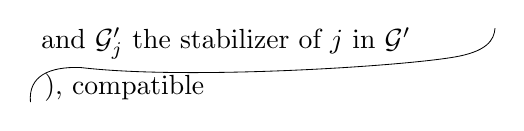
\begin{tikzpicture}[baseline=(base.base)]
\node[anchor=base west,inner sep=0] (base) at (0,0) {), compatible};
\node[anchor=base west,inner sep=0] at (-.04,.58) {\inserted{and $\mathcal G'_j$ the stabilizer of $j$ in $\mathcal G'$}};
\draw[line width=.3pt] (-.17,-.10) .. controls (-.20,.24) and (.08,.35) .. (.46,.34) .. controls (1.80,.18) and (4.48,.35) .. (5.20,.47) .. controls (5.63,.54) and (5.72,.69) .. (5.73,.84);
\end{tikzpicture}
with the actions of $\unsure{\mathcal E'|\Sigma'}$ on both
sides, \deleted{fitting into a family of
splittings modulo the action of $\pi_1$}
\[
\deleted{(26)\qquad\Psi^{\mathrm{ext}}=(\Psi_j^{\mathrm{ext}})_{j\in J}:\bigl(\widetilde{\mathfrak X}'(J)\unsure{\bigr)}\longrightarrow\operatorname{Hom}(\unsure{\mathcal G'|\mathcal G'_j},\unsure{\mathcal E'|\Sigma'})/\operatorname{Int}(\pi_1,\unsure{\mathcal E'|\Sigma'})}
\]
\deleted{also compatible with the action of $\unsure{\mathcal E'|\Sigma'}$\unsure{.}}

\textcircled{6} \uuline{Let us recapitulate.} We thus have: \deleted{$\mathfrak X$
scheme of finite type over $\overline{\mathbf Q}$, a divi}
\[
\mathrm I\quad\left\{\begin{array}{l}
\mathfrak X\text{ of finite type over }\overline{\mathbf Q}\\
D=\sum_{i\in I}D_i\text{ effective divisor on }\mathfrak X\text{ with}\\
\qquad\text{simple components, }\mathfrak X\text{ smooth at the maximal points}\\
\qquad\text{of }\operatorname{supp}D\\
J\underset{\text{\unsure{\uline{finite}}}}{\subset}\mathfrak X'(\overline{\mathbf Q}),\quad\text{where }\mathfrak X'=\mathfrak X-D
\end{array}\right.
\]
We set\margin{(}
\[
\mathrm{II}\quad\left\{\begin{array}{l}
\mathcal G'=\text{group of automorphisms of the \inserted{absolute} scheme }\mathfrak X\\
\qquad\text{which preserves }D\text{ and }J\\
G'=\text{subgroup of }\mathcal G'\text{ consisting of the }\overline{\mathbf Q}\text{-automorphisms}\\
\mathbf T(\overline{\mathbf Q})=\varprojlim_n\mu_n(\overline{\mathbf Q})\\[1ex]
\Gamma=\operatorname{Gal}(\overline{\mathbf Q}/\mathbf Q)
\end{array}\right.
\]
\mspage{8}
